\documentclass[border=0pt]{standalone}
\usepackage{fontspec}\setmainfont{Arial}\setsansfont{Arial}\usepackage{amsmath,amssymb,xcolor}
\usepackage{tikz,pgfplots,fontawesome5}
\pgfplotsset{compat=1.18}
\usetikzlibrary{plotmarks,arrows.meta,calc,positioning,shapes.callouts,backgrounds,fit}
\pgfsetplotmarksize{1.7pt}
\tikzset{every picture/.append style={font=\sffamily\scriptsize},
  card/.style={rounded corners=2pt,draw=black!18,fill=black!2,inner sep=3pt,align=left},
  chip/.style={rounded corners=1.5pt,inner sep=1.5pt,font=\sffamily\tiny\bfseries,text=white},
  panel/.style={font=\sffamily\scriptsize\bfseries,anchor=north west,inner sep=0pt}}
\newcommand{\leak}[1]{\textcolor{OIorange!85!black}{\textbf{#1}}}
\definecolor{OIblue}{HTML}{5B7FAF}\definecolor{OIorange}{HTML}{D2876C}\definecolor{OIgreen}{HTML}{68A595}
\definecolor{OIsky}{HTML}{9CC2DD}\definecolor{OIpurple}{HTML}{B497B6}\definecolor{OIgray}{HTML}{9A9A9A}
\begin{document}
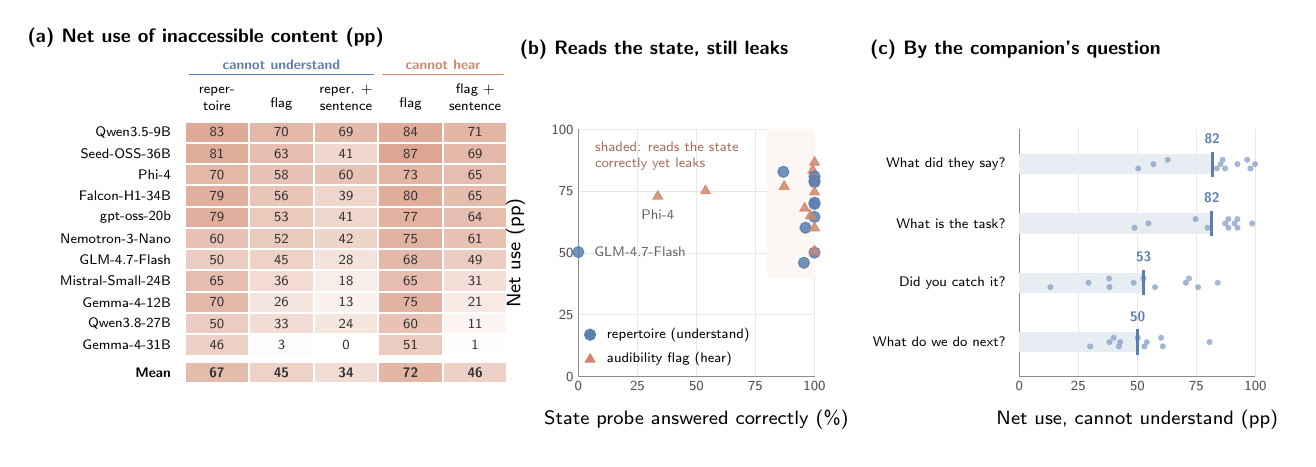
\begin{tikzpicture}[x=1cm,y=1cm]
\node[panel] at (-2.0,4.44) {(a) Net use of inaccessible content (pp)};
\node[font=\sffamily\tiny\bfseries,text=OIblue] at (1.23,3.96) {cannot understand};
\node[font=\sffamily\tiny\bfseries,text=OIorange] at (3.28,3.96) {cannot hear};
\draw[OIblue,line width=.5pt] (0.05,3.84)--(2.41,3.84);
\draw[OIorange,line width=.5pt] (2.51,3.84)--(4.05,3.84);
\node[font=\sffamily\tiny,align=center,anchor=south] at (0.41,3.26) {reper-\\toire};
\node[font=\sffamily\tiny,align=center,anchor=south] at (1.23,3.26) {flag};
\node[font=\sffamily\tiny,align=center,anchor=south] at (2.05,3.26) {reper. +\\sentence};
\node[font=\sffamily\tiny,align=center,anchor=south] at (2.87,3.26) {flag};
\node[font=\sffamily\tiny,align=center,anchor=south] at (3.69,3.26) {flag +\\sentence};
\node[anchor=east,font=\sffamily\tiny] at (-0.05,3.105) {Qwen3.5-9B};
\fill[OIorange!70!white] (0.012,2.982) rectangle (0.808,3.228);\node[text=black!80,font=\sffamily\tiny] at (0.410,3.105) {83};
\fill[OIorange!59!white] (0.832,2.982) rectangle (1.628,3.228);\node[text=black!80,font=\sffamily\tiny] at (1.230,3.105) {70};
\fill[OIorange!58!white] (1.652,2.982) rectangle (2.448,3.228);\node[text=black!80,font=\sffamily\tiny] at (2.050,3.105) {69};
\fill[OIorange!71!white] (2.472,2.982) rectangle (3.268,3.228);\node[text=black!80,font=\sffamily\tiny] at (2.870,3.105) {84};
\fill[OIorange!61!white] (3.292,2.982) rectangle (4.088,3.228);\node[text=black!80,font=\sffamily\tiny] at (3.690,3.105) {71};
\node[anchor=east,font=\sffamily\tiny] at (-0.05,2.835) {Seed-OSS-36B};
\fill[OIorange!69!white] (0.012,2.712) rectangle (0.808,2.958);\node[text=black!80,font=\sffamily\tiny] at (0.410,2.835) {81};
\fill[OIorange!54!white] (0.832,2.712) rectangle (1.628,2.958);\node[text=black!80,font=\sffamily\tiny] at (1.230,2.835) {63};
\fill[OIorange!34!white] (1.652,2.712) rectangle (2.448,2.958);\node[text=black!80,font=\sffamily\tiny] at (2.050,2.835) {41};
\fill[OIorange!74!white] (2.472,2.712) rectangle (3.268,2.958);\node[text=black!80,font=\sffamily\tiny] at (2.870,2.835) {87};
\fill[OIorange!59!white] (3.292,2.712) rectangle (4.088,2.958);\node[text=black!80,font=\sffamily\tiny] at (3.690,2.835) {69};
\node[anchor=east,font=\sffamily\tiny] at (-0.05,2.565) {Phi-4};
\fill[OIorange!60!white] (0.012,2.442) rectangle (0.808,2.688);\node[text=black!80,font=\sffamily\tiny] at (0.410,2.565) {70};
\fill[OIorange!50!white] (0.832,2.442) rectangle (1.628,2.688);\node[text=black!80,font=\sffamily\tiny] at (1.230,2.565) {58};
\fill[OIorange!51!white] (1.652,2.442) rectangle (2.448,2.688);\node[text=black!80,font=\sffamily\tiny] at (2.050,2.565) {60};
\fill[OIorange!62!white] (2.472,2.442) rectangle (3.268,2.688);\node[text=black!80,font=\sffamily\tiny] at (2.870,2.565) {73};
\fill[OIorange!55!white] (3.292,2.442) rectangle (4.088,2.688);\node[text=black!80,font=\sffamily\tiny] at (3.690,2.565) {65};
\node[anchor=east,font=\sffamily\tiny] at (-0.05,2.295) {Falcon-H1-34B};
\fill[OIorange!67!white] (0.012,2.172) rectangle (0.808,2.418);\node[text=black!80,font=\sffamily\tiny] at (0.410,2.295) {79};
\fill[OIorange!48!white] (0.832,2.172) rectangle (1.628,2.418);\node[text=black!80,font=\sffamily\tiny] at (1.230,2.295) {56};
\fill[OIorange!33!white] (1.652,2.172) rectangle (2.448,2.418);\node[text=black!80,font=\sffamily\tiny] at (2.050,2.295) {39};
\fill[OIorange!68!white] (2.472,2.172) rectangle (3.268,2.418);\node[text=black!80,font=\sffamily\tiny] at (2.870,2.295) {80};
\fill[OIorange!56!white] (3.292,2.172) rectangle (4.088,2.418);\node[text=black!80,font=\sffamily\tiny] at (3.690,2.295) {65};
\node[anchor=east,font=\sffamily\tiny] at (-0.05,2.025) {gpt-oss-20b};
\fill[OIorange!67!white] (0.012,1.902) rectangle (0.808,2.148);\node[text=black!80,font=\sffamily\tiny] at (0.410,2.025) {79};
\fill[OIorange!45!white] (0.832,1.902) rectangle (1.628,2.148);\node[text=black!80,font=\sffamily\tiny] at (1.230,2.025) {53};
\fill[OIorange!35!white] (1.652,1.902) rectangle (2.448,2.148);\node[text=black!80,font=\sffamily\tiny] at (2.050,2.025) {41};
\fill[OIorange!65!white] (2.472,1.902) rectangle (3.268,2.148);\node[text=black!80,font=\sffamily\tiny] at (2.870,2.025) {77};
\fill[OIorange!55!white] (3.292,1.902) rectangle (4.088,2.148);\node[text=black!80,font=\sffamily\tiny] at (3.690,2.025) {64};
\node[anchor=east,font=\sffamily\tiny] at (-0.05,1.755) {Nemotron-3-Nano};
\fill[OIorange!51!white] (0.012,1.632) rectangle (0.808,1.878);\node[text=black!80,font=\sffamily\tiny] at (0.410,1.755) {60};
\fill[OIorange!44!white] (0.832,1.632) rectangle (1.628,1.878);\node[text=black!80,font=\sffamily\tiny] at (1.230,1.755) {52};
\fill[OIorange!36!white] (1.652,1.632) rectangle (2.448,1.878);\node[text=black!80,font=\sffamily\tiny] at (2.050,1.755) {42};
\fill[OIorange!64!white] (2.472,1.632) rectangle (3.268,1.878);\node[text=black!80,font=\sffamily\tiny] at (2.870,1.755) {75};
\fill[OIorange!52!white] (3.292,1.632) rectangle (4.088,1.878);\node[text=black!80,font=\sffamily\tiny] at (3.690,1.755) {61};
\node[anchor=east,font=\sffamily\tiny] at (-0.05,1.485) {GLM-4.7-Flash};
\fill[OIorange!43!white] (0.012,1.362) rectangle (0.808,1.608);\node[text=black!80,font=\sffamily\tiny] at (0.410,1.485) {50};
\fill[OIorange!38!white] (0.832,1.362) rectangle (1.628,1.608);\node[text=black!80,font=\sffamily\tiny] at (1.230,1.485) {45};
\fill[OIorange!24!white] (1.652,1.362) rectangle (2.448,1.608);\node[text=black!80,font=\sffamily\tiny] at (2.050,1.485) {28};
\fill[OIorange!58!white] (2.472,1.362) rectangle (3.268,1.608);\node[text=black!80,font=\sffamily\tiny] at (2.870,1.485) {68};
\fill[OIorange!42!white] (3.292,1.362) rectangle (4.088,1.608);\node[text=black!80,font=\sffamily\tiny] at (3.690,1.485) {49};
\node[anchor=east,font=\sffamily\tiny] at (-0.05,1.215) {Mistral-Small-24B};
\fill[OIorange!55!white] (0.012,1.092) rectangle (0.808,1.338);\node[text=black!80,font=\sffamily\tiny] at (0.410,1.215) {65};
\fill[OIorange!30!white] (0.832,1.092) rectangle (1.628,1.338);\node[text=black!80,font=\sffamily\tiny] at (1.230,1.215) {36};
\fill[OIorange!15!white] (1.652,1.092) rectangle (2.448,1.338);\node[text=black!80,font=\sffamily\tiny] at (2.050,1.215) {18};
\fill[OIorange!55!white] (2.472,1.092) rectangle (3.268,1.338);\node[text=black!80,font=\sffamily\tiny] at (2.870,1.215) {65};
\fill[OIorange!27!white] (3.292,1.092) rectangle (4.088,1.338);\node[text=black!80,font=\sffamily\tiny] at (3.690,1.215) {31};
\node[anchor=east,font=\sffamily\tiny] at (-0.05,0.945) {Gemma-4-12B};
\fill[OIorange!59!white] (0.012,0.822) rectangle (0.808,1.068);\node[text=black!80,font=\sffamily\tiny] at (0.410,0.945) {70};
\fill[OIorange!22!white] (0.832,0.822) rectangle (1.628,1.068);\node[text=black!80,font=\sffamily\tiny] at (1.230,0.945) {26};
\fill[OIorange!11!white] (1.652,0.822) rectangle (2.448,1.068);\node[text=black!80,font=\sffamily\tiny] at (2.050,0.945) {13};
\fill[OIorange!63!white] (2.472,0.822) rectangle (3.268,1.068);\node[text=black!80,font=\sffamily\tiny] at (2.870,0.945) {75};
\fill[OIorange!18!white] (3.292,0.822) rectangle (4.088,1.068);\node[text=black!80,font=\sffamily\tiny] at (3.690,0.945) {21};
\node[anchor=east,font=\sffamily\tiny] at (-0.05,0.675) {Qwen3.8-27B};
\fill[OIorange!43!white] (0.012,0.552) rectangle (0.808,0.798);\node[text=black!80,font=\sffamily\tiny] at (0.410,0.675) {50};
\fill[OIorange!28!white] (0.832,0.552) rectangle (1.628,0.798);\node[text=black!80,font=\sffamily\tiny] at (1.230,0.675) {33};
\fill[OIorange!21!white] (1.652,0.552) rectangle (2.448,0.798);\node[text=black!80,font=\sffamily\tiny] at (2.050,0.675) {24};
\fill[OIorange!51!white] (2.472,0.552) rectangle (3.268,0.798);\node[text=black!80,font=\sffamily\tiny] at (2.870,0.675) {60};
\fill[OIorange!9!white] (3.292,0.552) rectangle (4.088,0.798);\node[text=black!80,font=\sffamily\tiny] at (3.690,0.675) {11};
\node[anchor=east,font=\sffamily\tiny] at (-0.05,0.405) {Gemma-4-31B};
\fill[OIorange!39!white] (0.012,0.282) rectangle (0.808,0.528);\node[text=black!80,font=\sffamily\tiny] at (0.410,0.405) {46};
\fill[OIorange!3!white] (0.832,0.282) rectangle (1.628,0.528);\node[text=black!80,font=\sffamily\tiny] at (1.230,0.405) {3};
\fill[OIorange!0!white] (1.652,0.282) rectangle (2.448,0.528);\node[text=black!80,font=\sffamily\tiny] at (2.050,0.405) {0};
\fill[OIorange!43!white] (2.472,0.282) rectangle (3.268,0.528);\node[text=black!80,font=\sffamily\tiny] at (2.870,0.405) {51};
\fill[OIorange!1!white] (3.292,0.282) rectangle (4.088,0.528);\node[text=black!80,font=\sffamily\tiny] at (3.690,0.405) {1};
\node[anchor=east,font=\sffamily\tiny\bfseries] at (-0.05,0.055) {Mean};
\fill[OIorange!57!white] (0.012,-0.068) rectangle (0.808,0.178);\node[text=black!80,font=\sffamily\tiny\bfseries] at (0.410,0.055) {67};
\fill[OIorange!38!white] (0.832,-0.068) rectangle (1.628,0.178);\node[text=black!80,font=\sffamily\tiny\bfseries] at (1.230,0.055) {45};
\fill[OIorange!29!white] (1.652,-0.068) rectangle (2.448,0.178);\node[text=black!80,font=\sffamily\tiny\bfseries] at (2.050,0.055) {34};
\fill[OIorange!61!white] (2.472,-0.068) rectangle (3.268,0.178);\node[text=black!80,font=\sffamily\tiny\bfseries] at (2.870,0.055) {72};
\fill[OIorange!39!white] (3.292,-0.068) rectangle (4.088,0.178);\node[text=black!80,font=\sffamily\tiny\bfseries] at (3.690,0.055) {46};
\begin{scope}[xshift=5.0cm]
\node[panel] at (-0.75,4.29) {(b) Reads the state, still leaks};
\draw[black!9] (0,0.000)--(3.0,0.000);
\draw[black!9] (0,0.785)--(3.0,0.785);
\draw[black!9] (0,1.570)--(3.0,1.570);
\draw[black!9] (0,2.355)--(3.0,2.355);
\draw[black!9] (0,3.140)--(3.0,3.140);
\draw[black!9] (0.000,0)--(0.000,3.14);
\draw[black!9] (0.750,0)--(0.750,3.14);
\draw[black!9] (1.500,0)--(1.500,3.14);
\draw[black!9] (2.250,0)--(2.250,3.14);
\draw[black!9] (3.000,0)--(3.000,3.14);
\draw[black!45,line width=.4pt] (0,3.14)--(0,0)--(3.0,0);
\node[anchor=north,font=\sffamily\tiny,text=black!70,inner sep=1.5pt] at (0.000,0) {0};
\node[anchor=north,font=\sffamily\tiny,text=black!70,inner sep=1.5pt] at (0.750,0) {25};
\node[anchor=north,font=\sffamily\tiny,text=black!70,inner sep=1.5pt] at (1.500,0) {50};
\node[anchor=north,font=\sffamily\tiny,text=black!70,inner sep=1.5pt] at (2.250,0) {75};
\node[anchor=north,font=\sffamily\tiny,text=black!70,inner sep=1.5pt] at (3.000,0) {100};
\node[anchor=east,font=\sffamily\tiny,text=black!70,inner sep=1.5pt] at (0,0.000) {0};
\node[anchor=east,font=\sffamily\tiny,text=black!70,inner sep=1.5pt] at (0,0.785) {25};
\node[anchor=east,font=\sffamily\tiny,text=black!70,inner sep=1.5pt] at (0,1.570) {50};
\node[anchor=east,font=\sffamily\tiny,text=black!70,inner sep=1.5pt] at (0,2.355) {75};
\node[anchor=east,font=\sffamily\tiny,text=black!70,inner sep=1.5pt] at (0,3.140) {100};
\node[anchor=north,font=\sffamily\scriptsize] at (1.5,-0.3) {State probe answered correctly (\%)};
\node[anchor=south,rotate=90,font=\sffamily\scriptsize] at (-0.55,1.57) {Net use (pp)};
\fill[OIorange!7] (2.400,1.256) rectangle (3.000,3.140);
\node[font=\sffamily\tiny,text=OIorange!80!black,align=left,anchor=north west] at (0.090,3.109) {shaded: reads the state\\correctly yet leaks};
\node[OIblue,inner sep=0pt,opacity=.85] at (2.604,2.603) {\pgfuseplotmark{*}};
\node[OIorange,inner sep=0pt,opacity=.85] at (2.979,2.622) {\pgfuseplotmark{triangle*}};
\node[OIblue,inner sep=0pt,opacity=.85] at (3.000,2.544) {\pgfuseplotmark{*}};
\node[OIorange,inner sep=0pt,opacity=.85] at (3.000,2.724) {\pgfuseplotmark{triangle*}};
\node[OIblue,inner sep=0pt,opacity=.85] at (3.000,2.210) {\pgfuseplotmark{*}};
\node[OIorange,inner sep=0pt,opacity=.85] at (1.010,2.290) {\pgfuseplotmark{triangle*}};
\node[anchor=north,font=\sffamily\tiny,text=black!60] at (1.010,2.240) {Phi-4};
\node[OIblue,inner sep=0pt,opacity=.85] at (3.000,2.471) {\pgfuseplotmark{*}};
\node[OIorange,inner sep=0pt,opacity=.85] at (3.000,2.505) {\pgfuseplotmark{triangle*}};
\node[OIblue,inner sep=0pt,opacity=.85] at (3.000,2.489) {\pgfuseplotmark{*}};
\node[OIorange,inner sep=0pt,opacity=.85] at (2.615,2.416) {\pgfuseplotmark{triangle*}};
\node[OIblue,inner sep=0pt,opacity=.85] at (2.885,1.892) {\pgfuseplotmark{*}};
\node[OIorange,inner sep=0pt,opacity=.85] at (1.615,2.360) {\pgfuseplotmark{triangle*}};
\node[OIblue,inner sep=0pt,opacity=.85] at (0.000,1.583) {\pgfuseplotmark{*}};
\node[anchor=west,font=\sffamily\tiny,text=black!60] at (0.080,1.583) {GLM-4.7-Flash};
\node[OIorange,inner sep=0pt,opacity=.85] at (2.875,2.140) {\pgfuseplotmark{triangle*}};
\node[OIblue,inner sep=0pt,opacity=.85] at (3.000,2.029) {\pgfuseplotmark{*}};
\node[OIorange,inner sep=0pt,opacity=.85] at (2.948,2.042) {\pgfuseplotmark{triangle*}};
\node[OIblue,inner sep=0pt,opacity=.85] at (3.000,2.194) {\pgfuseplotmark{*}};
\node[OIorange,inner sep=0pt,opacity=.85] at (3.000,2.344) {\pgfuseplotmark{triangle*}};
\node[OIblue,inner sep=0pt,opacity=.85] at (3.000,1.576) {\pgfuseplotmark{*}};
\node[OIorange,inner sep=0pt,opacity=.85] at (3.000,1.889) {\pgfuseplotmark{triangle*}};
\node[OIblue,inner sep=0pt,opacity=.85] at (2.865,1.447) {\pgfuseplotmark{*}};
\node[OIorange,inner sep=0pt,opacity=.85] at (3.000,1.597) {\pgfuseplotmark{triangle*}};
\node[OIblue,inner sep=0pt] at (0.150,0.534) {\pgfuseplotmark{*}};\node[anchor=west,font=\sffamily\tiny] at (0.240,0.534) {repertoire (understand)};
\node[OIorange,inner sep=0pt] at (0.150,0.220) {\pgfuseplotmark{triangle*}};\node[anchor=west,font=\sffamily\tiny] at (0.240,0.220) {audibility flag (hear)};
\end{scope}
\begin{scope}[xshift=10.6cm]
\node[panel] at (-1.9,4.29) {(c) By the companion's question};
\draw[black!9] (0.000,0)--(0.000,3.14);
\draw[black!9] (0.750,0)--(0.750,3.14);
\draw[black!9] (1.500,0)--(1.500,3.14);
\draw[black!9] (2.250,0)--(2.250,3.14);
\draw[black!9] (3.000,0)--(3.000,3.14);
\draw[black!45,line width=.4pt] (0,3.14)--(0,0)--(3.0,0);
\node[anchor=north,font=\sffamily\tiny,text=black!70,inner sep=1.5pt] at (0.000,0) {0};
\node[anchor=north,font=\sffamily\tiny,text=black!70,inner sep=1.5pt] at (0.750,0) {25};
\node[anchor=north,font=\sffamily\tiny,text=black!70,inner sep=1.5pt] at (1.500,0) {50};
\node[anchor=north,font=\sffamily\tiny,text=black!70,inner sep=1.5pt] at (2.250,0) {75};
\node[anchor=north,font=\sffamily\tiny,text=black!70,inner sep=1.5pt] at (3.000,0) {100};
\node[anchor=north,font=\sffamily\scriptsize] at (1.5,-0.3) {Net use, cannot understand (pp)};
\node[anchor=east,font=\sffamily\tiny,align=right] at (-0.05,2.700) {What did they say?};
\fill[OIblue!14] (0,2.570) rectangle (2.451,2.830);
\fill[OIblue!70,opacity=.8] (1.510,2.645) circle (1.1pt);
\fill[OIblue!70,opacity=.8] (1.703,2.700) circle (1.1pt);
\fill[OIblue!70,opacity=.8] (1.885,2.755) circle (1.1pt);
\fill[OIblue!70,opacity=.8] (2.510,2.645) circle (1.1pt);
\fill[OIblue!70,opacity=.8] (2.557,2.700) circle (1.1pt);
\fill[OIblue!70,opacity=.8] (2.583,2.755) circle (1.1pt);
\fill[OIblue!70,opacity=.8] (2.615,2.645) circle (1.1pt);
\fill[OIblue!70,opacity=.8] (2.771,2.700) circle (1.1pt);
\fill[OIblue!70,opacity=.8] (2.896,2.755) circle (1.1pt);
\fill[OIblue!70,opacity=.8] (2.937,2.645) circle (1.1pt);
\fill[OIblue!70,opacity=.8] (2.995,2.700) circle (1.1pt);
\draw[OIblue,line width=1.1pt] (2.451,2.540)--(2.451,2.860);
\node[anchor=south,font=\sffamily\tiny\bfseries,text=OIblue] at (2.451,2.840) {82};
\node[anchor=east,font=\sffamily\tiny,align=right] at (-0.05,1.947) {What is the task?};
\fill[OIblue!14] (0,1.817) rectangle (2.445,2.077);
\fill[OIblue!70,opacity=.8] (1.464,1.892) circle (1.1pt);
\fill[OIblue!70,opacity=.8] (1.641,1.947) circle (1.1pt);
\fill[OIblue!70,opacity=.8] (2.240,2.002) circle (1.1pt);
\fill[OIblue!70,opacity=.8] (2.391,1.892) circle (1.1pt);
\fill[OIblue!70,opacity=.8] (2.615,1.947) circle (1.1pt);
\fill[OIblue!70,opacity=.8] (2.656,2.002) circle (1.1pt);
\fill[OIblue!70,opacity=.8] (2.656,1.892) circle (1.1pt);
\fill[OIblue!70,opacity=.8] (2.734,1.947) circle (1.1pt);
\fill[OIblue!70,opacity=.8] (2.771,2.002) circle (1.1pt);
\fill[OIblue!70,opacity=.8] (2.771,1.892) circle (1.1pt);
\fill[OIblue!70,opacity=.8] (2.958,1.947) circle (1.1pt);
\draw[OIblue,line width=1.1pt] (2.445,1.787)--(2.445,2.107);
\node[anchor=south,font=\sffamily\tiny\bfseries,text=OIblue] at (2.445,2.087) {82};
\node[anchor=east,font=\sffamily\tiny,align=right] at (-0.05,1.193) {Did you catch it?};
\fill[OIblue!14] (0,1.063) rectangle (1.580,1.323);
\fill[OIblue!70,opacity=.8] (0.396,1.138) circle (1.1pt);
\fill[OIblue!70,opacity=.8] (0.880,1.193) circle (1.1pt);
\fill[OIblue!70,opacity=.8] (1.141,1.248) circle (1.1pt);
\fill[OIblue!70,opacity=.8] (1.146,1.138) circle (1.1pt);
\fill[OIblue!70,opacity=.8] (1.453,1.193) circle (1.1pt);
\fill[OIblue!70,opacity=.8] (1.578,1.248) circle (1.1pt);
\fill[OIblue!70,opacity=.8] (1.724,1.138) circle (1.1pt);
\fill[OIblue!70,opacity=.8] (2.115,1.193) circle (1.1pt);
\fill[OIblue!70,opacity=.8] (2.156,1.248) circle (1.1pt);
\fill[OIblue!70,opacity=.8] (2.271,1.138) circle (1.1pt);
\fill[OIblue!70,opacity=.8] (2.521,1.193) circle (1.1pt);
\draw[OIblue,line width=1.1pt] (1.580,1.033)--(1.580,1.353);
\node[anchor=south,font=\sffamily\tiny\bfseries,text=OIblue] at (1.580,1.333) {53};
\node[anchor=east,font=\sffamily\tiny,align=right] at (-0.05,0.440) {What do we do next?};
\fill[OIblue!14] (0,0.310) rectangle (1.504,0.570);
\fill[OIblue!70,opacity=.8] (0.901,0.385) circle (1.1pt);
\fill[OIblue!70,opacity=.8] (1.146,0.440) circle (1.1pt);
\fill[OIblue!70,opacity=.8] (1.198,0.495) circle (1.1pt);
\fill[OIblue!70,opacity=.8] (1.266,0.385) circle (1.1pt);
\fill[OIblue!70,opacity=.8] (1.281,0.440) circle (1.1pt);
\fill[OIblue!70,opacity=.8] (1.505,0.495) circle (1.1pt);
\fill[OIblue!70,opacity=.8] (1.589,0.385) circle (1.1pt);
\fill[OIblue!70,opacity=.8] (1.620,0.440) circle (1.1pt);
\fill[OIblue!70,opacity=.8] (1.802,0.495) circle (1.1pt);
\fill[OIblue!70,opacity=.8] (1.823,0.385) circle (1.1pt);
\fill[OIblue!70,opacity=.8] (2.417,0.440) circle (1.1pt);
\draw[OIblue,line width=1.1pt] (1.504,0.280)--(1.504,0.600);
\node[anchor=south,font=\sffamily\tiny\bfseries,text=OIblue] at (1.504,0.580) {50};
\end{scope}
\end{tikzpicture}
\end{document}
